\chapter{Determinants and Eigenvalues}
\label{C:D&E}

\normalsize

In Section~\ref{S:det2x2} we introduced determinants for $2\times 2$
matrices $A$.  There we showed that the determinant of $A$
is nonzero if and only if $A$ is invertible.  In Section~\ref{S:evchp} 
we saw that the eigenvalues of $A$ are the roots of its 
characteristic polynomial, and that its characteristic polynomial
is just the determinant of a related matrix, namely, 
$p_A(\lambda) = \det(A-\lambda I_2)$. 

In Section~\ref{S:det} we generalize the concept of determinants to
$n\times n$ matrices, and in Section~\ref{S:eig} we use determinants 
to show that every $n\times n$ matrix has exactly $n$ eigenvalues --- 
the roots of its characteristic polynomial.  Properties of eigenvalues 
are also discussed in detail in Section~\ref{S:eig}.\index{eigenvalue}
Certain details concerning determinants are deferred to Appendix~\ref{A:det}.



\Section{Determinants} 
\label{S:det}
 
There are several equivalent ways to introduce determinants --- none of which 
are easily motivated.  We prefer to define determinants through the properties 
they satisfy rather than by formula.  These properties actually enable us to 
compute determinants of $n\times n$ matrices where $n>3$, which further 
justifies the approach. Later on, we will give an inductive formula 
\Ref{e:inductdet} for computing the determinant. 
 
\begin{Def}  \label{D:determinants}
A {\em determinant\/} of a square $n\times n$ matrix $A$ is a real
number that satisfies the following three properties:
\begin{itemize} 
\item[(a)]  If $A=(a_{ij})$ is lower 
triangular\index{matrix!lower triangular}, then
the determinant of $A$ is the product of the diagonal entries;
that is,
\[
\det(A) = a_{11}\cdot\cdots\cdot a_{nn}.
\]
\item[(b)]  $\det(A^t)=\det(A)$\index{matrix!transpose}.
\item[(c)]  Let $B$ be an $n\times n$ matrix.  
Then
\begin{equation} \label{e:detproduct}
\det(AB) = \det(A)\det(B).
\end{equation}
\end{itemize}
\end{Def} \index{determinant}

\begin{thm}  \label{T:determinants}
There exists a unique determinant function satisfying the three
properties of Definition~\ref{D:determinants}.
\end{thm}\index{determinant!uniqueness}

We will show that it is possible to compute the determinant of
any $n\times n$ matrix using Definition~\ref{D:determinants}.
Here we present a few examples:

\begin{lemma}
Let $A$ be an $n\times n$ matrix.
\begin{itemize}
\item[(a)]   Let $c\in\R$ be a scalar.  Then $\det(cA) = c^n\det(A)$.
\item[(b)] If all of the entries in either a row or a column of $A$ are 
zero, then $\det(A)=0$.
\end{itemize}
\end{lemma}

\proof  (a) Note that Definition~\ref{D:determinants}(a) implies that 
$\det(cI_n)=c^n$.  It follows from \Ref{e:detproduct} that
\[
\det(cA) = \det(cI_n A) = \det(cI_n)\det(A) = c^n\det(A).
\]

(b)  Definition~\ref{D:determinants}(b) implies that it suffices to prove 
this assertion when one row of $A$ is zero.  Suppose that the $i^{th}$ row 
of $A$ is zero.  Let $J$ be an $n\times n$ 
diagonal matrix with a $1$ in every diagonal entry except the $i^{th}$ 
diagonal entry which is $0$.  A matrix calculation shows that $JA=A$. 
It follows from Definition~\ref{D:determinants}(a) that $\det(J)=0$ and 
from \Ref{e:detproduct} that $\det(A)=0$.  \qed 



\subsection*{Determinants of $2\times 2$ Matrices}
\index{determinant!of $2\times 2$ matrices} 
 
Before discussing how to compute determinants, we discuss the
special case of $2\times 2$ matrices.  Recall from \Ref{D:determinant} of 
Section~\ref{S:det2x2} that when 
\[
A=\left(\begin{array}{cc} a & b\\c & d \end{array}\right)
\]
we defined 
\begin{equation}  \label{e:determinantn=2}
\det(A)=ad-bc.
\end{equation}
We check that \Ref{e:determinantn=2} satisfies the three
properties in Definition~\ref{D:determinants}.  Observe that when
$A$ is lower triangular, then $b=0$ and $\det(A)=ad$.  So (a) is
satisfied.  It is straightforward to verify (b).  We already
verified (c) in Chapter~\ref{chap:matrices}, Proposition~\ref{propdet}.

It is less obvious perhaps --- but true nonetheless --- that the
three properties of $\det(A)$ actually force the determinant of
$2\times 2$ matrices to be given by formula
\Ref{e:determinantn=2}. We begin by showing that
Definition~\ref{D:determinants} implies that 
\begin{equation}  \label{e:detswap}
\det \left(\begin{array}{cc} 0 & 1\\1 & 0 \end{array}\right)=-1.
\end{equation}
We verify this by observing that 
\begin{equation} \label{e:swapdecomp}
\left(\begin{array}{cc} 0 & 1\\1 & 0 \end{array}\right) =
\left(\begin{array}{cr} 1 & -1\\0 & 1 \end{array}\right)
\left(\begin{array}{cc} 1 & 0\\1 & 1 \end{array}\right)
\left(\begin{array}{cr} 1 & 0\\0 & -1 \end{array}\right)
\left(\begin{array}{cc} 1 & 1\\0 & 1 \end{array}\right).
\end{equation}
Hence property (c), (a) and (b) imply that
\[
\det \left(\begin{array}{cc} 0 & 1\\1 & 0 \end{array}\right) =
1\cdot 1\cdot (-1) \cdot 1 = -1.
\]
It is helpful to interpret the matrices in \Ref{e:swapdecomp} as
elementary row operations\index{elementary row operations}.  
Then \Ref{e:swapdecomp} states that
swapping two rows in a $2\times 2$ matrix is the same as
performing the following row operations in order:
\begin{itemize}
\item        add the $2^{nd}$ row to the  $1^{st}$ row;
\item        multiply the $2^{nd}$ row by $-1$; 
\item        add the $1^{st}$ row to the $2^{nd}$ row; and  
\item        subtract the $2^{nd}$ row from the $1^{st}$ row.
\end{itemize}
 
Suppose that $d\neq 0$.  Then 
\[
A=\left(\begin{array}{cc} a & b\\c & d \end{array}\right) =
\left(\begin{array}{cc} 1 & \frac{b}{d}\\0 & 1 \end{array}\right)
\left(\begin{array}{cc} \frac{ad-bc}{d} & 0\\c & d
\end{array}\right). 
\]
It follows from properties (c), (b) and (a) that
\[
\det(A) = \frac{ad-bc}{d}d = ad-bc,
\]
as claimed.
 
Now suppose that $d=0$ and note that 
\[
A=\left(\begin{array}{cc} a & b\\c & 0 \end{array}\right) = 
\left(\begin{array}{cc} 0 & 1\\1 & 0 \end{array}\right)
\left(\begin{array}{cc} c & 0\\a & b \end{array}\right).
\]
Using \Ref{e:detswap} we see that 
\[
\det(A) = -\det \left(\begin{array}{cc} c & 0\\a & b
\end{array}\right) = -bc,
\]
as desired. 
 
We have verified that the only possible determinant function for
$2\times 2$ matrices is the determinant function defined by
\Ref{e:determinantn=2}. 
 



\subsection*{Row Operations are Invertible Matrices} 
\index{elementary row operations}

\begin{prop}  \label{P:ERO}
Let $A$ and $B$ be $m\times n$ matrices where $B$ is obtained from $A$ by
a single elementary row operation.  Then there exists an invertible 
$m\times m$ matrix $R$ such that $B=RA$.
\end{prop} 

\proof  First consider multiplying the $j^{th}$ row of $A$ by the
nonzero constant $c$.  Let $R$ be the diagonal matrix whose
$j^{th}$ entry on the diagonal is $c$ and whose other diagonal 
entries are $1$.  Then the matrix $RA$ is just the matrix obtained from 
$A$ by multiplying the $j^{th}$ row of $A$ by $c$.  Note that $R$ is
invertible when $c\neq 0$ and that $R\inv$ is the diagonal
matrix whose $j^{th}$ entry is $\frac{1}{c}$ and whose other
diagonal entries are $1$.  For example
\[
\left(\begin{array}{ccc} 1 & 0 & 0\\ 0 & 1 & 0 \\ 0 & 0 & 2\end{array}\right)
\left(\begin{array}{ccc} a_{11} & a_{12} & a_{13}\\ a_{21} & a_{22} & a_{23}
 \\ a_{31} & a_{32} & a_{33} \end{array}\right) =
\left(\begin{array}{ccc} a_{11} & a_{12} & a_{13}\\ a_{21} & a_{22} & a_{23}
 \\ 2a_{31} & 2a_{32} & 2a_{33} \end{array}\right),
\]
multiplies the $3^{rd}$ row by $2$.

Next we show that the elementary row operation that swaps two
rows may also be thought of as matrix multiplication.  Let
$R=(r_{kl})$ be the matrix that deviates from the identity matrix
by changing in the four entries:
\begin{eqnarray*}
r_{ii} & = & 0 \\
r_{jj} & = & 0\\
r_{ij} & = & 1 \\
r_{ji} & = & 1
\end{eqnarray*}
A calculation shows that $RA$ is the matrix obtained from $A$ by
swapping the $i^{th}$ and $j^{th}$ rows.  For example,
\[
\left(\begin{array}{ccc} 0 & 0 & 1\\ 0 & 1 & 0 \\ 1 & 0 & 0\end{array}\right)
\left(\begin{array}{ccc} a_{11} & a_{12} & a_{13}\\ a_{21} & a_{22} & a_{23}
 \\ a_{31} & a_{32} & a_{33} \end{array}\right) =
\left(\begin{array}{ccc} a_{31} & a_{32} & a_{33}\\ a_{21} & a_{22} & a_{23}
 \\  a_{11} & a_{12} & a_{13} \end{array}\right),
\]
which swaps the $1^{st}$ and $3^{rd}$ rows.  Another calculation
shows that $R^2=I_n$ and hence that $R$ is invertible since
$R\inv=R$.  

Finally, we claim that adding $c$ times the $i^{th}$ row of $A$
to the $j^{th}$ row of $A$ can be viewed as matrix
multiplication.  Let $E_{k\ell}$ be the matrix all of whose
entries are $0$ except for the entry in the $k^{th}$ row and
$\ell^{th}$ column which is $1$.  Then $R=I_n+cE_{ij}$ has the
property that $RA$ is the matrix obtained by adding $c$ times
the $j^{th}$ row of $A$ to the $i^{th}$ row.  We can verify by
multiplication that $R$ is invertible and that
$R\inv=I_n-cE_{ij}$.  More precisely,
\[
(I_n+cE_{ij})(I_n-cE_{ij})=I_n+cE_{ij}-cE_{ij}-c^2E_{ij}^2=I_n,
\]
since $E_{ij}^2 = O$ for $i\not= j$.  For example,
\begin{eqnarray*}
(I_3 + 5E_{12})A &  = & \left(\begin{array}{ccc} 1 & 5 & 0\\ 0 & 1 & 0 \\ 0 & 0 & 1\end{array}\right)
\left(\begin{array}{ccc} a_{11} & a_{12} & a_{13}\\ a_{21} & a_{22} & a_{23}
 \\ a_{31} & a_{32} & a_{33} \end{array}\right) \\ & = & 
\left(\begin{array}{ccc} a_{11}+5a_{21} & a_{12}+5a_{22} & a_{13}+5a_{23} \\ 
a_{21} & a_{22} & a_{23} \\ a_{31} & a_{32} & a_{33} \end{array}\right),
\end{eqnarray*}
adds $5$ times the $2^{nd}$ row to the $1^{st}$ row.   \qed

\subsubsection*{Determinants of Elementary Row Matrices}

\begin{lemma}  \label{L:detelemrowmat}
\begin{itemize}
\item[(a)] The determinant of a swap matrix is $-1$.
\item[(b)] The determinant of the matrix that adds a multiple
of one row to another is $1$.
\item[(c)] The determinant of the matrix that multiplies one
row by $c$ is $c$.
\end{itemize}
\end{lemma}  \index{determinant}
 
\proof The matrix that swaps the $i^{th}$ row with the $j^{th}$
row is the matrix whose nonzero elements are $a_{kk}=1$ where
$k\neq i,j$ and $a_{ij}=1=a_{ji}$.  Using a similar argument as
in \Ref{e:detswap} we see that the determinants of these
matrices are equal to $-1$.
 
The matrix that adds a multiple of one row to another is
triangular (either upper or lower) and has $1$'s on the
diagonal.  Thus property (a) in Definition~\ref{D:determinants}
implies that the determinants of
these matrices are equal to $1$.
 
Finally, the matrix that multiplies the $i^{th}$ row by $c\neq
0$ is a diagonal matrix all of whose diagonal entries are $1$
except for $a_{ii}=c$.  Again property (a) implies that the
determinant of this matrix is $c\neq 0$. \qed


\subsection*{Computation of Determinants}
\index{determinant!computation}

We now show how to compute the determinant of any $n\times n$ matrix $A$ 
using elementary row operations and Definition~\ref{D:determinants}.  It 
follows from Proposition~\ref{P:ERO} that every elementary row operation 
on $A$ may be performed by premultiplying $A$ by an elementary row matrix. 

For each matrix $A$ there is a unique 
reduced echelon form\index{echelon form!reduced} matrix
$E$ and a sequence of elementary row matrices $R_1\ldots R_s$
such that \index{elementary row operations}
\begin{equation}  \label{e:rowreduction}
E = R_s\cdots R_1A.
\end{equation}
It follows from Definition~\ref{D:determinants}(c) that we can
compute the determinant of $A$ once we know the determinants of
reduced echelon form matrices and the determinants of elementary
row matrices.  In particular
\begin{equation}  \label{e:detformula}
\det(A) = \det(E)/(\det(R_1)\cdots\det(R_s)).
\end{equation}

It is easy to compute the determinant of any matrix in reduced echelon 
form using Definition~\ref{D:determinants}(a) since all reduced echelon 
form $n\times n$ matrices are upper triangular.  Lemma~\ref{L:detelemrowmat}  
tells us how to compute the determinants of elementary row matrices.  This 
discussion proves: 
\begin{prop}
If a determinant function exists for $n\times n$ matrices, then it is unique. 
\index{determinant!uniqueness}
\end{prop}

We still need to show that determinant functions exist when $n>2$.  More 
precisely, we know that the reduced echelon form matrix $E$ is uniquely 
defined from $A$ (Chapter~\ref{lineq}, Theorem~\ref{uniquerowechelon}), but 
there is more than one way to perform elementary row operations on $A$ to 
get to $E$.  Thus, we can write $A$ in the form \Ref{e:detformula} in many 
different ways, and these different decompositions might lead to different 
values for $\det A$.  (They don't.)

\subsubsection*{An Example of Determinants by Row Reduction}
\index{row!reduction}

As a practical matter we row reduce a square matrix $A$ by 
premultiplying $A$ by an elementary row matrix $R_j$.  Thus 
\begin{equation} \label{e:pracdet}
\det(A) = \frac{1}{\det(R_j)} \det (R_j A).
\end{equation}
We use this approach to compute the determinant of the 
$4\times 4$ matrix 
\[
A = \left(\begin{array}{rrrr} 0 & 2 & 10 & -2 \\ 1 & 2 & 4 & 0\\
1 & 6 & 1 & -2 \\ 2 & 1 & 1 & 0 \end{array}\right).
\]
The idea is to use \Ref{e:pracdet} to keep track of the 
determinant while row reducing $A$ to upper triangular form. 
For instance, swapping rows changes the sign of the determinant; 
so
\[
\det(A) = -\det\left(\begin{array}{rrrr} 1 & 2 & 4 & 0\\ 0 & 2 & 10 & -2 \\
1 & 6 & 1 & -2 \\ 2 & 1 & 1 & 0 \end{array}\right).
\]
Adding multiples of one row to another leaves the determinant
unchanged; so
\[
\det(A) = -\det\left(\begin{array}{rrrr} 1 & 2 & 4 & 0\\ 0 & 2 & 10 & -2 \\
0 & 4 & -3 & -2 \\ 0 & -3 & -7 & 0 \end{array}\right).
\]
Multiplying a row by a scalar $c$ corresponds to an elementary 
row matrix whose determinant is $c$.  To make sure that we do not 
change the value of $\det(A)$, we have to divide the determinant by 
$c$ as we multiply a row of $A$ by $c$. So as we divide the second 
row of the matrix by $2$, we multiply the whole result by $2$, obtaining   
\[
\det(A) = -2\det\left(\begin{array}{rrrr} 1 & 2 & 4 & 0\\ 0 & 1 & 5 & -1 \\
0 & 4 & -3 & -2 \\ 0 & -3 & -7 & 0 \end{array}\right).
\] 
We continue row reduction by zeroing out the last two entries in
the $2^{nd}$ column, obtaining
\[
\det(A) = -2\det\left(\begin{array}{rrrr} 1 & 2 & 4 & 0\\ 0 & 1 & 5 & -1 \\
0 & 0 & -23 & 2 \\ 0 & 0 & 8 & -3 \end{array}\right)
= 46\det\left(\begin{array}{rrrr} 1 & 2 & 4 & 0\\ 0 & 1 & 5 & -1 \\
0 & 0 & 1 & -\frac{2}{23} \\ 0 & 0 & 8 & -3 \end{array}\right).
\] 
Thus
\[
\det(A) = 46\det\left(\begin{array}{rrrr} 1 & 2 & 4 & 0\\ 0 & 1 & 5 & -1 \\
0 & 0 & 1 & -\frac{2}{23} \\ 0 & 0 & 0 & -\frac{53}{23} \end{array}\right)
= -106.
\]  

\subsubsection*{Determinants and Inverses}
\index{inverse}

We end this subsection with an important observation about the
determinant function.  This observation generalizes to dimension
$n$ Corollary~\ref{C:2x2invert} of Chapter~\ref{chap:matrices}. 
\begin{thm}  \label{T:detandinv}
An $n\times n$ matrix $A$ is invertible if and only if $\det(A)\neq 0$.
Moreover, if $A\inv$ exists, then 
\begin{equation}  \label{E:detinv}
\det A\inv = \frac{1}{\det A}.
\end{equation}
\end{thm} \index{invertible}
 
\proof  If $A$ is invertible, then 
\[
\det(A)\det(A\inv) = \det(AA\inv) = \det(I_n) =1.
\]
Thus $\det(A)\neq 0$ and \Ref{E:detinv} is valid. In particular, the 
determinants of elementary row matrices are nonzero, since they are all
invertible. (This point was proved by direct calculation in
Lemma~\ref{L:detelemrowmat}.)
 
If $A$ is singular, then $A$ is row equivalent to a non-identity
reduced echelon form matrix $E$ whose determinant is zero (since
$E$ is upper triangular and its last diagonal entry is zero).
So it follows from
\Ref{e:rowreduction} that 
\[
0=\det(E) = \det(R_1)\cdots\det(R_s)\det(A)
\]
Since $\det(R_j)\neq 0$, it follows that $\det(A)=0$.  \qed

\begin{cor}
If the rows of an $n\times n$ matrix $A$ are linearly dependent (for example,
if one row of $A$ is a scalar multiple of another row of $A$), then 
$\det(A)=0$.
\end{cor}


\subsection*{An Inductive Formula for Determinants} 
\index{determinant!inductive formula for}
 
In this subsection we present an inductive formula for the
determinant --- that is, we assume that the determinant is known
for square $(n-1)\times(n-1)$ matrices and use this formula to
define the determinant for $n\times n$ matrices.  This inductive formula
is called {\em expansion by cofactors\/}.
 
Let $A=(a_{ij})$ be an $n\times n$ matrix.  Let $A_{ij}$ be the
$(n-1)\times(n-1)$ matrix formed from $A$ by deleting the
$i^{th}$ row and the $j^{th}$ column.  The matrices $(-1)^{i+j}A_{ij}$ are
called {\em cofactor\/} \index{cofactor} matrices of $A$.  

Inductively we define the determinant of an $n\times n$ matrix $A$ by:
\begin{eqnarray}  
\det(A) & = & \sum^n_{j=1} (-1)^{1+j}a_{1j}\det(A_{1j}) \nonumber
\\  & = &
a_{11}\det(A_{11})-a_{12}\det(A_{12})+\cdots+(-1)^{n+1}a_{1n}\det(A_{1n}).
    \label{e:inductdet}
\end{eqnarray} \index{determinant}
In Appendix~\ref{A:det} we show that the determinant function defined by 
\Ref{e:inductdet} satisfies all properties of a determinant function.
Formula \Ref{e:inductdet} is also called {\em expansion by cofactors along 
the $1^{st}$ row\/}, since the $a_{1j}$ are taken from the $1^{st}$ row 
of $A$.  Since $\det(A)=\det(A^t)$, it follows that if \Ref{e:inductdet} is 
valid as an inductive definition of determinant, then expansion by cofactors 
along the $1^{st}$ column is also valid.  That is,
\begin{equation}  \label{e:inductdetc}
\det(A) = 
a_{11}\det(A_{11})-a_{21}\det(A_{21})+\cdots+(-1)^{n+1}a_{n1}\det(A_{n1}).
\end{equation} 

We now explore some of the consequences of this definition, beginning 
with determinants of small matrices.  For example, 
Definition~\ref{D:determinants}(a) implies that the determinant of a 
$1\times 1$ matrix is just
\[
\det(a) = a.
\]
Therefore, using \Ref{e:inductdet}, the determinant of a $2\times
2$ matrix is:
\[
\det\left(\begin{array}{cc} a_{11} & a_{12}\\a_{21} & a_{22}
\end{array}\right) = a_{11}\det(a_{22}) - a_{12}\det(a_{21}) =
a_{11}a_{22} - a_{12}a_{21},
\]
which is just the formula for determinants of $2\times 2$
\index{determinant!of $2\times 2$ matrices}
matrices given in \Ref{e:determinantn=2}. 
 
Similarly, we can now find a formula for the determinant of
$3\times 3$ matrices $A$ as follows.
\begin{eqnarray} 
\det(A) & = & a_{11}
\det \left(\begin{array}{cc} a_{22} & a_{23}\\a_{32} & a_{33}
\end{array}\right) 
- a_{12}
\det \left(\begin{array}{cc} a_{21} & a_{23}\\a_{31} & a_{33}
\end{array}\right) 
+ a_{13}
\det\left(\begin{array}{cc} a_{21} & a_{22}\\a_{31} & a_{32}
\end{array}\right) \nonumber \\
 & & \label{e:det3} \\
& = & a_{11}a_{22}a_{33} + a_{12}a_{23}a_{31} + a_{13}a_{21}a_{32}
- a_{11}a_{23}a_{32} - a_{12}a_{21}a_{33} - a_{13}a_{22}a_{31}. \nonumber
\end{eqnarray}  

As an example, compute
\[
\det\left(\begin{array}{rrr} 2 & 1 & 4\\ 1 & -1 & 3\\ 5 & 6 & -2
\end{array}\right) 
\]
using formula \Ref{e:det3} as
\[
2(-1)(-2) + 1\cdot3\cdot5 + 4\cdot6\cdot1 -4(-1)5 -3\cdot6\cdot2
- (-2)1\cdot1  = 4+15+24+20 -36 +2 = 29. 
\]

There is a visual mnemonic for remembering how to compute the six
terms in formula \Ref{e:det3} for the determinant of 
$3\times 3$ matrices\index{determinant!of $3\times 3$ matrices}.
Write the matrix as a $3\times 5$ array by repeating the first 
two columns, as shown in bold face in Figure~\ref{F:det3}:
\index{determinant!computation}
\begin{figure}[htb]
           \centerline{%
            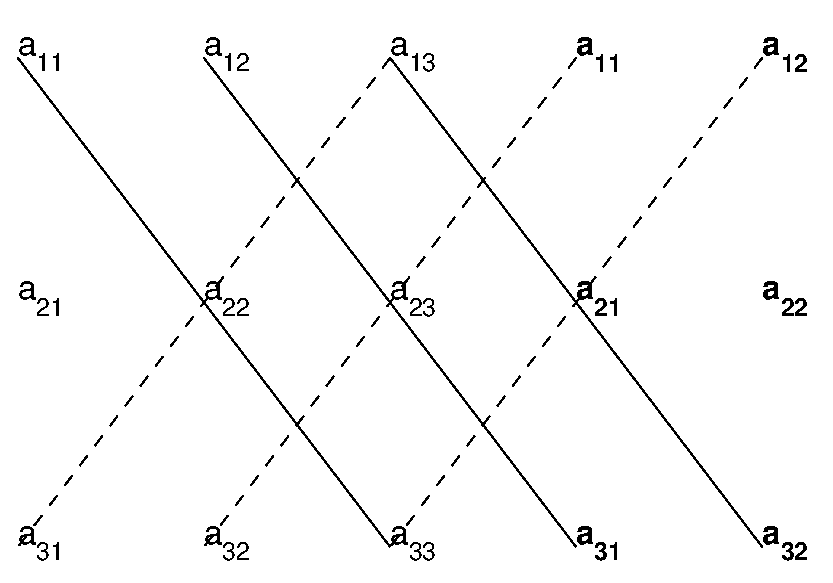
\psfig{file=figures/det3.eps,height=2.5in}}
           \caption{Mnemonic for computation of determinants of 
		$3\times 3$ matrices.}
           \label{F:det3}
\end{figure}
Then add the product of terms connected by solid lines sloping down and 
to the right and subtract the products of terms connected by dashed lines 
sloping up and to the right.  Warning: this nice crisscross algorithm 
for computing determinants of $3\times 3$ matrices does not generalize 
to $n\times n$ matrices.
 
When computing determinants of $n\times n$ matrices when $n>3$,
it is usually more efficient to compute the determinant using row
reduction rather than by using formula \Ref{e:inductdet}.  In the
appendix to this chapter, Section~\ref{A:det}, we verify that formula 
\Ref{e:inductdet} actually satisfies the three properties of a determinant, 
thus completing the proof of Theorem~\ref{T:determinants}.  

An interesting and useful formula for reducing the effort in 
computing determinants is given by the following formula.
\begin{lemma} \label{L:detblockdiag}
Let $A$ be an $n\times n$ matrix of the form
\[
A=\mattwo{B}{0}{C}{D},
\]
where $B$ is a $k\times k$ matrix and $D$ is an $(n-k)\times(n-k)$
matrix.  Then
\[
\det(A)=\det(B)\det(D).
\]
\end{lemma}

\proof We prove this result using \Ref{e:inductdet} coupled with 
induction. Assume that this lemma is valid or all $(n-1)\times
(n-1)$ matrices of the appropriate form.  Now use
\Ref{e:inductdet} to compute
\begin{eqnarray*}
\det(A) & = & a_{11}\det(A_{11})-a_{12}\det(A_{12}) + \cdots\pm
a_{1n}\det(A_{1n}) \\
& = &  b_{11}\det(A_{11})-b_{12}\det(A_{12}) + \cdots\pm
b_{1k}\det(A_{1k}).
\end{eqnarray*}
Note that the cofactor matrices $A_{1j}$ are obtained from $A$
by deleting the $1^{st}$ row and the $j^{th}$ column.  These
matrices all have the form
\[
A_{1j} = \mattwo{B_{1j}}{0}{C_j}{D},
\]
where $C_j$ is obtained from $C$ by deleting the $j^{th}$
column. By induction on $k$
\[
\det(A_{1j}) = \det(B_{1j})\det(D).
\]
It follows that 
\begin{eqnarray*}
\det(A) & = & \left(b_{11}\det(B_{11})-b_{12}\det(B_{12}) + \cdots\pm
b_{1k}\det(B_{1k})\right)\det(D) \\
& = & \det(B)\det(D),
\end{eqnarray*}
as desired.  \qed


\subsection*{Determinants in \Matlab}
\index{determinant!in \protect\Matlab}

The determinant function has been preprogrammed in \Matlab and
is quite easy to use.  For example, typing {\tt e8\_1\_11} will
load the matrix
\begin{equation*}  \label{e:A4x4}
A = \left(\begin{array}{rrrr}
     1   &  2  &   3  &   0\\
     2   &  1  &   4  &   1\\
    -2   & -1  &   0  &   1\\
    -1   &  0  &  -2  &   3  \end{array} \right).
\end{equation*}
To compute the determinant of $A$ just type {\tt det(A)} and
obtain the answer \index{\computer!det}
\begin{verbatim}
ans =
   -46
\end{verbatim}

Alternatively, we can use row reduction techniques in \Matlab to
compute the determinant of $A$ --- just to test the theory that
we have developed.  Note that to compute the determinant we do
not need to row reduce to 
reduced echelon form\index{echelon form!reduced} --- we need only
reduce to an upper triangular matrix.  This can always be done
by successively adding multiples of one row to another --- an
operation that does not change the determinant.  For example,
to clear the entries in the $1^{st}$ column below the $1^{st}$
row, type
\begin{verbatim}
A(2,:) = A(2,:) - 2*A(1,:);
A(3,:) = A(3,:) + 2*A(1,:); 
A(4,:) = A(4,:) + A(1,:)
\end{verbatim}
obtaining 
\begin{verbatim}
A =
     1     2     3     0
     0    -3    -2     1
     0     3     6     1
     0     2     1     3
\end{verbatim}
To clear the $2^{nd}$ column below the $2^{nd}$ row type 
\begin{verbatim}
A(3,:) = A(3,:) + A(2,:);A(4,:) = A(4,:) - A(4,2)*A(2,:)/A(2,2)\end{verbatim}
obtaining
\begin{verbatim}
A =
    1.0000    2.0000    3.0000         0
         0   -3.0000   -2.0000    1.0000
         0         0    4.0000    2.0000
         0         0   -0.3333    3.6667
\end{verbatim}
Finally, to clear the entry $(4,3)$ type
\begin{verbatim}
A(4,:) = A(4,:) -A(4,3)*A(3,:)/A(3,3)\end{verbatim}
to obtain
\begin{verbatim}
A =
    1.0000    2.0000    3.0000         0
         0   -3.0000   -2.0000    1.0000
         0         0    4.0000    2.0000
         0         0         0    3.8333
\end{verbatim}
To evaluate the determinant of $A$, which is now an upper
triangular matrix, type
\begin{verbatim}
A(1,1)*A(2,2)*A(3,3)*A(4,4)\end{verbatim}
obtaining
\begin{verbatim}
ans =
   -46
\end{verbatim}
as expected.

\EXER

\TEXER


\noindent  In Exercises~\ref{c10.1.1a} -- \ref{c10.1.1c} compute the 
determinants of the given matrix.
\begin{exercise} \label{c10.1.1a}
$A = \left(\begin{array}{rrr} -2 & 1 & 0 \\ 4 & 5& 0 \\ 1 & 0 & 2
\end{array} \right)$.
\end{exercise} 
\begin{exercise} \label{c10.1.1b}
$B = \left(\begin{array}{rrrr} 1 & 0 & 2 & 3 \\ -1 & -2 & 3 & 2
\\ 4 & -2 & 0 & 3 \\ 1 & 2 & 0 & -3 \end{array} \right)$.
\end{exercise}
\begin{exercise} \label{c10.1.1c}
$C = \left(\begin{array}{rrrrr} 2 & 1 & -1 & 0 & 0 \\ 1 & -2 & 3
& 0 & 0 \\ -3 & 2 & -2 & 0 & 0 \\ 1 & 1 & -1 & 2 & 4 \\ 0 & 2 &
3 & -1 & -3 \end{array} \right)$.
\end{exercise}

\begin{exercise} \label{c10.1.2}
Find $\det(A\inv)$ where 
$A = \left(\begin{array}{rrr} -2 & -3 & 2 \\ 4 & 1 & 3 \\ -1 & 1 & 1
\end{array} \right)$. 
\end{exercise}

\begin{exercise} \label{c10.1.3}
Show that the determinants of similar $n\times n$ matrices are
equal. 
\end{exercise}

\noindent In Exercises~\ref{c10.1.4} -- \ref{c10.1.5b} use row reduction 
to compute the determinant of the given matrix.
\begin{exercise} \label{c10.1.4}
$A = \left(\begin{array}{rrr} -1 & -2 & 1 \\ 3 & 1 & 3 \\ -1 & 1 & 1
\end{array} \right)$. 
\end{exercise}
\begin{exercise} \label{c10.1.5a}
$B = \left(\begin{array}{rrrr} 1 & 0 & 1 & 0 \\ 0 & 1 & 0 & -1 \\
1 & 0 & -1 & 0 \\ 0 & 1 & 0 & 1 \end{array}\right)$.
\end{exercise}
\begin{exercise} \label{c10.1.5b}
$C = \left(\begin{array}{rrrr} 1 & 2 & 0 & 1 \\ 0 & 2 & 1 & 0 \\
-2 & -3 & 3 & -1 \\ 1 & 0 & 5 & 2 \end{array}\right)$.
\end{exercise}

\begin{exercise} \label{c10.1.6}
Let 
\[
A = \left(\begin{array}{rrr} 2 & -1 & 0 \\ 0 & 3 & 0 \\ 1 & 5 & 3
\end{array} \right)  \AND
B = \left(\begin{array}{rrr} 2 & 0 & 0 \\ 0 & -1 & 0 \\ 0 & 0 & 3
\end{array} \right).
\]
\begin{itemize}
\item[(a)] For what values of $\lambda$ is  $\det(\lambda A-B)=0$?
\item[(b)] Is there a vector $x$ for which $Ax=Bx$?
\end{itemize}
\end{exercise}

\noindent In Exercises~\ref{c10.1.a7a} -- \ref{c10.1.a7b} verify 
that the given matrix has determinant $-1$.
\begin{exercise} \label{c10.1.a7a}
$A = \left( \begin{array}{rrr}
1  &  0  &  0\\
0  &  0  &  1\\
0  &  1  &  0
\end{array} \right)$.
\end{exercise}
\begin{exercise} \label{c10.1.a7b}
$B = \left( \begin{array}{rrr}
 0 &   0 &   1\\
 0 &   1 &   0\\
 1 &   0 &   0
\end{array} \right)$.
\end{exercise}


\begin{exercise} \label{c10.1.b7a}
Compute the cofactor matrices $A_{13}, A_{22}, A_{21}$ when 
$A = \left( \begin{array}{rrr}
 3 & 2 & -4\\
 0 & 1 & 5\\
 0 & 0 & 6\end{array} \right)$.
\end{exercise}
\begin{exercise} \label{c10.1.b7b}
Compute the cofactor matrices $B_{11}, B_{23}, B_{43}$ when
$B = \left( \begin{array}{rrrr}
 0 & 2 & -4 & 5\\
 -1 & 7 & -2 & 10\\
 0 & 0 & 0  & -1\\
3 & 4 & 2 & -10
\end{array} \right)$.
\end{exercise}

\begin{exercise} \label{c10.1.c7}
Find values of $\lambda$ where the determinant of the matrix
\[
A_\lambda = \left( \begin{array}{ccr}
 \lambda -1 & 0 & -1\\
 0 & \lambda -1 & 1\\
-1 & 1 & \lambda 
\end{array} \right)
\]
vanishes.  
\end{exercise}

\begin{exercise}  \label{c10.1.c8} 
Suppose that two $n\times p$ matrices $A$ and $B$ are row
equivalent. \index{row!equivalent} Show that there is an invertible
$n\times n$ matrix $P$ such that $B = PA$.
\end{exercise}

\begin{exercise} \label{c10.1.c9}
Let $A$ be an invertible $n\times n$ matrix and let $b\in\R^n$ be a column 
vector. Let $B_j$ be the $n\times n$ matrix obtained from $A$ by replacing the 
$j^{th}$ column of $A$ by the vector $b$.  Let $x=(x_1,\ldots,x_n)^t$ be the 
unique solution to $Ax=b$. Then Cramer's rule \index{Cramer's rule} states that
\begin{equation}  \label{E:cramer2}
x_j = \frac{\det(B_j)}{\det(A)}.
\end{equation}
Prove Cramer's rule.  {\bf Hint}: Let $A_j$ be the $j^{th}$ column of $A$ so
that $A_j = Ae_j$.  Show that 
\[
B_j = A (e_1|\cdots|e_{j-1}|x|e_{j+1}|\cdots|e_n).
\]
Using this product, compute the determinant of $B_j$ and verify \Ref{E:cramer2}.
\end{exercise}

\Section{Eigenvalues} \label{S:eig} 
 
In this section we discuss how to find eigenvalues for an
$n\times n$ matrix $A$.  This discussion parallels the
discussion for $2\times 2$ matrices given in
Section~\ref{S:evchp}.  As we noted in that section, $\lambda$
is a real eigenvalue of $A$ if there exists a nonzero
eigenvector $v$ such that
\begin{equation}  \label{e:eigen}
Av = \lambda v.
\end{equation}
It follows that the matrix $A-\lambda I_n$ is 
singular\index{singular} since
\[
(A-\lambda I_n)v = 0.
\]
Theorem~\ref{T:detandinv} implies that 
\[
\det(A-\lambda I_n) = 0.
\]
With these observations in mind, we can make the following definition.
\begin{Def}   \label{D:charpoly}
Let $A$ be an $n\times n$ matrix.  The {\em characteristic polynomial\/} 
of $A$ is:
\[
p_A(\lambda) = \det(A-\lambda I_n).
\]  \index{characteristic polynomial}
\end{Def}

In Theorem~\ref{T:charpolyn} we show that $p_A(\lambda)$ is indeed a 
polynomial of degree $n$ in $\lambda$.  Note here that the roots of 
\index{characteristic polynomial!roots}
$p_A$ are the {\em eigenvalues\/} of $A$. As we
discussed, the real eigenvalues\index{eigenvalue!real} 
of $A$ are roots of the
characteristic polynomial.  \index{eigenvalue} Conversely, if
$\lambda$ is a real root of $p_A$, then
Theorem~\ref{T:detandinv} states that the matrix $A-\lambda I_n$
is singular and therefore that there exists a nonzero vector $v$
such that \Ref{e:eigen} is satisfied.  Similarly, by using this
extended algebraic definition of eigenvalues we allow the
possibility of complex eigenvalues\index{eigenvalue!complex}.  
The complex analog of
Theorem~\ref{T:detandinv} shows that if $\lambda$ is a complex
eigenvalue, then there exists a nonzero complex $n$-vector $v$
such that \Ref{e:eigen} is satisfied.

\begin{exam} \label{E:triangular}
Let $A$ be an $n\times n$ lower triangular matrix.  Then the
diagonal entries are the eigenvalues of $A$.  {\rm We verify
this statement as follows.  \index{matrix!lower triangular}
\[
A-\lambda I_n = \left(\begin{array}{ccc} a_{11}-\lambda &  & 0 \\
 &  \ddots &  \\ (*) & & a_{nn}-\lambda \end{array}\right).
\]
Since the determinant of a triangular matrix is the product of
the diagonal entries, it follows that 
\begin{equation}  \label{e:triangpoly}
p_A(\lambda) = (a_{11}-\lambda)\cdots(a_{nn}-\lambda),
\end{equation}
and hence that the diagonal entries of $A$ are roots of the 
characteristic polynomial. A similar argument works if $A$ is
upper triangular.}
\end{exam}  
 
It follows from \Ref{e:triangpoly} that the characteristic
polynomial of a triangular matrix
\index{characteristic polynomial!of triangular matrices}
is a polynomial of degree $n$ and that
\begin{equation}  \label{e:leadingterm}
p_A(\lambda) = (-1)^n \lambda^n + b_{n-1}\lambda^{n-1} + \cdots +b_0.
\end{equation}
for some real constants $b_0, \ldots, b_{n-1}$. In fact, this
statement is true in general.  

\begin{thm}  \label{T:charpolyn}
Let $A$ be an $n\times n$ matrix.  Then $p_A$ is a polynomial of
degree $n$ of the form \Ref{e:leadingterm}.
\end{thm} \index{characteristic polynomial}

\proof Let $C$ be an $n\times n$ matrix whose entries have
the form $c_{ij}+d_{ij}\lambda$.  Then $\det(C)$ is a polynomial
in $\lambda$ of degree at most $n$.  We verify this statement by
induction. It is easily verified when $n=1$, since then
$C=(c+d\lambda)$ for some real numbers $c$ and $d$. Then
$\det(C)=c+d\lambda$ which is a polynomial of degree at most
one.  (It may have degree zero, if $d=0$.) So assume that this
statement is true for $(n-1)\times (n-1)$ matrices. Recall from
\Ref{e:inductdet} that 
\[
\det(C) = (c_{11}+d_{11}\lambda)\det(C_{11})
+\cdots+(-1)^{n+1}(c_{1n}+d_{1n}\lambda)\det(C_{1n}).
\]    
By induction each of the determinants $C_{1j}$ is a polynomial
of degree at most $n-1$.  It follows that multiplication by
$c_{1j}+d_{1j}\lambda$ yields a polynomial of degree at most $n$
in $\lambda$.  Since the sum of polynomials of degree at most
$n$ is a polynomial of degree at most $n$, we have verified our
assertion.

Since $A-\lambda I_n$ is a matrix whose entries have the
desired form, it follows that $p_A(\lambda)$ is a polynomial of
degree at most $n$ in $\lambda$.  To complete the proof of this
theorem we need to show that the coefficient of $\lambda^n$ is
$(-1)^n$.  Again, we verify this statement by induction.  This
statement is easily verified for $1\times 1$ matrices --- we
assume that it is true for $(n-1)\times (n-1)$ matrices.  Again
use \Ref{e:inductdet} to compute
\[
\det(A-\lambda I_n) = (a_{11}-\lambda)\det(B_{11})-a_{12}\det(B_{12}) 
+\cdots+(-1)^{n+1}a_{1n}\det(B_{1n}).
\]
where $B_{1j}$ are the cofactor \index{cofactor} matrices of
$A-\lambda I_n$.  Using our previous observation all of the
terms $\det(B_{1j})$ are polynomials of degree at most $n-1$.
Thus, in this expansion, the only term that can contribute a
term of degree $n$ is:
\[
-\lambda\det(B_{11}).
\]
Note that the cofactor matrix $B_{11}$ is the $(n-1)\times
(n-1)$ matrix
\[
B_{11} = A_{11} -\lambda I_{n-1},
\]
where $A_{11}$ is the first cofactor matrix of the matrix $A$.
By induction, $\det(B_{11})$ is a polynomial of degree $n-1$ with
leading term $(-1)^{n-1}\lambda^{n-1}$.  Multiplying this
polynomial by $-\lambda$ yields a polynomial of degree $n$ with
the correct leading term.  \qed

\subsection*{General Properties of Eigenvalues}

The {\em fundamental theorem of algebra\/} \index{fundamental
theorem of algebra} states that every polynomial of degree $n$
has exactly $n$ roots (counting multiplicity).  For example, the 
quadratic formula shows that 
every quadratic polynomial has exactly two roots.  In general, the proof 
of the fundamental theorem is not easy and is certainly beyond the 
limits of this course.  Indeed, the difficulty in proving the {\em
fundamental theorem of algebra\/} is in proving that a
polynomial $p(\lambda)$ of degree $n>0$ has one (complex) root.
Suppose that $\lambda_0$ is a root of $p(\lambda)$; that is,
suppose that $p(\lambda_0)=0$. Then it is easy to show that
\begin{equation}  \label{e:factoring}
p(\lambda) = (\lambda-\lambda_0)q(\lambda)
\end{equation}
for some polynomial $q$ of degree $n-1$.  So once we know that
$p$ has a root, then we can argue by induction to prove that $p$
has $n$ roots.  

Recall that a polynomial need not have any real roots. For
example, the polynomial $p(\lambda)=\lambda^2+1$ has no real
roots, since $p(\lambda)> 0$ for all real $\lambda$.  This
polynomial does have two complex roots $\pm i =\pm\sqrt{-1}$.  

However, a polynomial with real coefficients has either real
roots or complex roots that come in complex conjugate pairs.  To
verify this statement, we need to show that if $\lambda_0$ is a
complex root of $p(\lambda)$, then so is $\overline{\lambda_0}$.
We claim that 
\[
p(\overline{\lambda})=\overline{p(\lambda)}.
\]
To verify this point, suppose that
\[
p(\lambda) = c_n\lambda^n + c_{n-1}\lambda^{n-1} + \cdots + c_0,
\]
where each $c_j\in\R$.  Then
\[
\overline{p(\lambda)}
=\overline{c_n\lambda^n + c_{n-1}\lambda^{n-1} + \cdots + c_0} 
= c_n\overline{\lambda}^n + c_{n-1}\overline{\lambda}^{n-1} + \cdots + c_0
= p(\overline{\lambda})
\]
If $\lambda_0$ is a root of $p(\lambda)$, then
\[
p(\overline{\lambda_0}) = \overline{p(\lambda_0)}=\overline{0}=0.
\]
Hence $\overline{\lambda_0}$ is also a root of $p$.

It follows that 
\begin{thm}  \label{T:eigens}
Every (real) $n\times n$ matrix $A$ has exactly $n$ eigenvalues
$\lambda_1,\ldots,\lambda_n$.  These eigenvalues are either real
or complex conjugate pairs.  Moreover,
\begin{enumerate}
\item[(a)] $p_A(\lambda) = (\lambda_1-\lambda)\cdots(\lambda_n-\lambda)$,
\item[(b)] $\det(A) = \lambda_1\cdots\lambda_n$.
\end{enumerate}
\end{thm} \index{eigenvalue}\index{eigenvalue!existence}
\index{determinant}

\proof Since the characteristic polynomial $p_A$ is a polynomial
of degree $n$ with real coefficients, the first part of the
theorem follows from the preceding discussion. In particular, it follows
from \Ref{e:factoring} that 
\[
p_A(\lambda) = c(\lambda_1-\lambda)\cdots(\lambda_n-\lambda),
\]
for some constant $c$.  Formula \Ref{e:leadingterm} implies that
$c=1$ --- which proves (a).  Since $p_A(\lambda)=\det(A-\lambda I_n)$, 
it follows that $p_A(0)=\det(A)$.  Thus (a) implies 
that $p_A(0)=\lambda_1\cdots\lambda_n$, thus proving (b).  \qed

The eigenvalues of a matrix do not have to be different.  For
example, consider the extreme case of a strictly triangular
matrix $A$.  Example~\ref{E:triangular} shows that all of the
eigenvalues of $A$ are zero. 

We now discuss certain properties of eigenvalues.  
\begin{cor}  \label{C:eig=0}
Let $A$ be an $n\times n$ matrix. Then $A$ is invertible if and
only if zero is {\em not\/} an eigenvalue of $A$.
\end{cor}  \index{invertible}

\proof The proof follows from Theorem~\ref{T:detandinv} and
Theorem~\ref{T:eigens}(b). \qed 

\begin{lemma} 
Let $A$ be a singular $n\times n$ matrix.  Then the null space of $A$
is the span of all eigenvectors whose associated eigenvalue is zero.
\end{lemma} \index{null space}\index{singular}

\proof An eigenvector $v$ of $A$ has eigenvalue zero if and only
if 
\[
Av=0.
\]
This statement is valid if and only if $v$ is in the null space
of $A$. \qed



\begin{thm}  \label{T:inveig}
Let $A$ be an invertible $n\times n$ matrix with eigenvalues 
$\lambda_1,\cdots,\lambda_n$.  Then the eigenvalues of 
$A\inv$ are $\lambda_1\inv,\cdots,\lambda_n\inv$.
\end{thm}  \index{invertible}\index{eigenvalue!of inverse}

\proof  We claim that  
\[
p_A(\lambda) = (-1)^n \det(A) \lambda^n p_{A\inv}(\frac{1}{\lambda}).
\]
It then follows that $\frac{1}{\lambda}$ is an eigenvalue for
$A\inv$ for each eigenvalue $\lambda$ of $A$.  This makes sense,
since the eigenvalues of $A$ are nonzero. 

Compute:
\begin{eqnarray*}
(-1)^n \det(A) \lambda^n p_{A\inv}(\frac{1}{\lambda}) & = &
 (-\lambda)^n \det(A)\det(A\inv-\frac{1}{\lambda}I_n) \\
& = & \det(-\lambda A)\det(A\inv-\frac{1}{\lambda}I_n)\\
& = & \det(-\lambda A (A\inv-\frac{1}{\lambda}I_n))\\
& = & \det(A-\lambda I_n) \\
& = & p_A(\lambda),
\end{eqnarray*}
which verifies the claim.  \qed

\begin{thm}  \label{T:similareigen}
Let $A$ and $B$ be similar $n\times n$ matrices.  Then
\[
p_A = p_B,
\]
and hence the eigenvalues of $A$ and $B$ are identical.
\end{thm}  \index{similar}

\proof  Since $B$ and $A$ are similar, there exists an 
invertible $n\times n$ matrix $S$ such that $B=S\inv AS$.  It 
follows that 
\[
\det(B-\lambda I_n) = \det(S\inv AS-\lambda I_n)
= \det(S\inv(A-\lambda I_n)S) = \det(A-\lambda I_n),
\]
which verifies that $p_A=p_B$.  \qed

Recall that the {\em trace\/}\index{trace} of an 
$n\times n$ matrix $A$ is
the sum of the diagonal entries of $A$; that is
\[
{\rm tr}(A) = a_{11} +\cdots+ a_{nn}.
\]
We state without proof the following theorem:
\begin{thm} \label{T:tracen}
Let $A$ be an $n\times n$ matrix with eigenvalues
$\lambda_1,\ldots,\lambda_n$.  Then
\[
{\rm tr}(A) = \lambda_1 + \cdots + \lambda_n.
\]
\end{thm}

It follows from Theorem~\ref{T:similareigen} that the traces of
similar matrices are equal.


\subsection*{\Matlab Calculations}

The commands for computing characteristic polynomials and
eigenvalues of square matrices are straightforward in \Matlab.
In particular, for an $n\times n$ matrix $A$, the \Matlab command
 {\tt poly(A)} returns the coefficients of $(-1)^np_A(\lambda)$.

For example, reload the $4\times 4$ matrix $A$ of \Ref{e:A4x4}
by typing {\tt e8\_1\_11}.  The characteristic polynomial of $A$ is
found by typing
\begin{verbatim}
poly(A)
\end{verbatim} \index{\computer!poly}
to obtain
\begin{verbatim}
ans =
    1.0000   -5.0000   15.0000  -10.0000  -46.0000
\end{verbatim} 
Thus the characteristic polynomial of $A$ is:
\[
p_A(\lambda) = \lambda^4 -5\lambda^3+15\lambda^2-10\lambda-46.
\]
The eigenvalues of $A$ are found by typing {\tt eig(A)} and
obtaining
\begin{verbatim}
ans =
  -1.2224          
   1.6605 + 3.1958i
   1.6605 - 3.1958i
   2.9014 
\end{verbatim}
Thus $A$ has two real eigenvalues and one complex conjugate pair
of eigenvalues.  Note that \Matlab has preprogrammed not only
the algorithm for finding the characteristic polynomial, but
also numerical routines for finding the roots of the
characteristic polynomial.

The trace of $A$ is found by typing {\tt trace(A)} and obtaining
\begin{verbatim} 
ans =
     5
\end{verbatim} \index{\computer!trace}

Using the \Matlab command {\tt sum} we can verify the statement
of Theorem~\ref{T:tracen}.  Indeed {\tt sum(v)} computes the sum 
of the components of the vector $v$ and typing
\begin{verbatim}
sum(eig(A))
\end{verbatim}
\index{\computer!sum}
we obtain the answer {\tt 5.0000}, as expected.

\EXER

\TEXER

\noindent In Exercises~\ref{c10.2.1a} -- \ref{c10.2.1b} determine the 
characteristic polynomial and the eigenvalues of the given matrices.
\begin{exercise} \label{c10.2.1a}
$A = \left(\begin{array}{rrr} -9 & -2 & -10 \\ 3 & 2 & 3 \\
8 & 2 & 9 \end{array}\right)$. 
\end{exercise}
\begin{exercise} \label{c10.2.1b}
$B = \left(\begin{array}{rrrr} 2 & 1 & -5 & 2 \\ 1 & 2 & 13 & 2 \\
0 & 0 & 3 & -1 \\ 0 & 0 & 1 & 1 \end{array}\right)$.
\end{exercise}

\begin{exercise} \label{c10.2.2}
Find a basis for the eigenspace of 
\[
A = \left(\begin{array}{rrr} 3 & 1 & -1 \\ -1 & 1 & 1 \\ 2 & 2 & 0 
\end{array}\right)
\]
corresponding to the eigenvalue $\lambda=2$.
\end{exercise}

\begin{exercise} \label{c10.2.3}
Consider the matrix  
\[
A = \left(\begin{array}{rrr} -1 & 1 & 1 \\ 1 & -1 & 1 \\ 1 & 1 & -1 
\end{array}\right).
\]
\begin{itemize}
\item[(a)] Verify that the characteristic polynomial of $A$ is
 $p_\lambda(A)=(\lambda-1)(\lambda+2)^2$.
\item[(b)] Show that $(1,1,1)$ is an eigenvector of $A$ corresponding to 
$\lambda=1$.
\item[(c)] Show that $(1,1,1)$ is orthogonal to every eigenvector 
of $A$ corresponding to the eigenvalue $\lambda=-2$.
\end{itemize}
\end{exercise}

\begin{exercise} \label{c10.2.4}
Consider the matrix $A=\mattwo{8}{5}{-10}{-7}$.
\begin{itemize}
\item[(a)] Find the eigenvalues and eigenvectors of $A$.
\item[(b)] Show that the eigenvectors found in (a) form a basis for $\R^2$.
\item[(c)] Find the coordinates of the vector $(x_1,x_2)$ relative to the 
basis in part (b).
\end{itemize}
\end{exercise}

\begin{exercise} \label{c10.2.5}
Find the characteristic polynomial and the eigenvalues of 
\[
A = \left(\begin{array}{rrr} -1 & 2 & 2 \\ 2 & 2 & 2 \\ -3 & -6 & -6 
\end{array}\right).
\]
Find eigenvectors corresponding to each of the three eigenvalues.
\end{exercise}

\begin{exercise} \label{c10.2.6}
Let $A$ be an $n\times n$ matrix.  Suppose that 
\[
A^2 + A + I_n = 0.
\]
Prove that $A$ is invertible.
\end{exercise}

\noindent In Exercises~\ref{c10.2.7a} -- \ref{c10.2.7b} decide whether 
the given statements are {\em true\/} or {\em false\/}. If the 
statements are false, give a counterexample; if the statements are true, 
give a proof.
\begin{exercise} \label{c10.2.7a}
If the eigenvalues of a $2\times 2$ matrix are equal to $1$,
then the four entries of that matrix are each less than $500$.
\end{exercise}
\begin{exercise} \label{c10.2.7b}
The trace of the product of two $n\times n$ matrices is the
product of the traces.
\end{exercise}

\begin{exercise} \label{c10.2.8}
When $n$ is odd show that every real $n\times n$ matrix has a real
eigenvalue. 
\end{exercise}

\CEXER

\noindent In Exercises~\ref{c10.2.9a} -- \ref{c10.2.9b}, use \Matlab to 
compute (a) the eigenvalues, traces, and characteristic polynomials of 
the given matrix.  (b) Use the results from part (a) to confirm 
Theorems~\ref{T:inveig} and \ref{T:tracen}.
\begin{exercise} \label{c10.2.9a}
\begin{equation*}
A=\left( \begin{array}{rrrrr}
      -12 & -19 &  -3 &  14 &   0\\
      -12 &  10 &  14 & -19 &   8\\
        4 &  -2 &   1 &   7 &  -3\\
       -9 &  17 & -12 &  -5 &  -8\\
      -12 &  -1 &   7 &  13 & -12
\end{array} \right).
\end{equation*}
\end{exercise}
\begin{exercise} \label{c10.2.9b}
\begin{equation*}
B=\left( \begin{array}{rrrrrr}
      -12 &  -5 &  13 &  -6 & -5 &  12\\
        7 &  14 &   6 &   1 &  8 &  18\\
       -8 &  14 &  13 &   9 &  2 &   1\\
        2 &   4 &   6 &  -8 & -2 &  15\\
      -14 &   0 &  -6 &  14 &  8 & -13\\
        8 &  16 &  -8 &   3 &  5 &  19
\end{array} \right).
\end{equation*}
\end{exercise}

\begin{exercise} \label{c10.2.10}
Use \Matlab to compute the characteristic polynomial of the following
matrix:
\[
A = \left( \begin{array}{rrr}
 4 & -6 & 7\\
 2 & 0 & 5\\
-10 & 2 & 5
\end{array} \right)
\]
Denote this polynomial by $p_A(\lambda) = 
-(\lambda^3 + p_2 \lambda^2 + p_1 \lambda + p_0)$.  Then compute
the matrix
\[
B = -(A^3 + p_2 A^2 + p_1 A + p_0 I).
\]
What do you observe?  In symbols $B=p_A(A)$.  Compute the matrix $B$ for
examples of other square matrices $A$ and determine whether or not 
your observation was an accident.
\end{exercise}




\Sec{*Appendix: Existence of Determinants}{APPENDIX: EXISTENCE OF DETERMINANTS}
%\Section{Appendix: Existence of Determinants}
\label{A:det}

The purpose of this appendix is to verify the inductive
definition of determinant \Ref{e:inductdet}. We have already
shown that if a determinant function exists, then it is unique.
We also know that the determinant function exists for $1\times
1$ matrices. So we assume by induction that the determinant function
exists for $(n-1)\times(n-1)$ matrices and prove that the
inductive definition gives a determinant function for $n\times
n$ matrices.  \index{determinant}

Recall that $A_{ij}$ is the cofactor matrix obtained from $A$ by
deleting the $i^{th}$ row and $j^{th}$ column --- so $A_{ij}$ is
an $(n-1)\times(n-1)$ matrix.  The inductive definition is:
\index{determinant!inductive formula for}
\[
D(A) = a_{11}\det(A_{11})-a_{12}\det(A_{12})+\cdots 
+(-1)^{n+1}a_{1n}\det(A_{1n}).
\] \index{cofactor}
We use the notation $D(A)$ to remind us that we have not yet
verified that this definition satisfies properties (a)-(c) of
Definition~\ref{D:determinants}.  In this appendix we verify these
properties after assuming that the inductive definition
satisfies properties (a)-(c) for $(n-1)\times (n-1)$ matrices.
For emphasis, we use the notation $\det$ to indicate the
determinant of square matrices of size less than $n$.

Property (a) is easily verified for $D(A)$ since if $A$ is lower
triangular, then
\[
D(A) = a_{11}\det(A_{11}) = a_{11}a_{22}\cdots a_{nn}
\]
by induction.

Before verifying that $D$ satisfies properties (b) and (c) of a
determinant, we prove:
\begin{lemma}
Let $E$ be a elementary row matrix and let $B$ be any $n\times
n$ matrix.   Then
\begin{equation} \label{e:proddetE}
D(EB) = D(E) D(B)
\end{equation} 
\end{lemma}

\proof We verify \Ref{e:proddetE} for each of the three types of
elementary row operations. \index{elementary row operations}

\noindent (I) Suppose that $E$ multiplies the $i^{th}$ row by a
nonzero scalar $c$.  If $i>1$, then the cofactor matrix
$(EA)_{1j}$ is obtained from the cofactor matrix $A_{1j}$ by
multiplying the $(i-1)^{st}$ row by $c$.  By induction,
$\det(EA)_{1j}= c\det(A_{1j})$ and $D(EA)=cD(A)$.  On the other
hand, $D(E)=\det(E_{11})=c$.  So \Ref{e:proddetE} is verified in
this instance.  If $i=1$, then the $1^{st}$ row of $EA$ is
$(ca_{11},\ldots,ca_{1n})$ from which it is easy to verify
\Ref{e:proddetE}.

\noindent (II) Next suppose that $E$ adds a multiple $c$ of the
$i^{th}$ row to the $j^{th}$ row.  We note that $D(E)=1$.  When
$j>1$ then $D(E)=\det(E_{11})=1$ by induction.  When $j=1$ then
$D(E)= \det(E_{11})\pm c\det(E_{1i})=\det(I_{n-1})\pm
c\det(E_{1i})$. But $E_{1i}$ is strictly upper triangular and
$\det(E_{1i})=0$.  Thus $D(E)=1$. 

If $i>1$ and $j>1$, then the result $D(EA)=D(A)=D(E)D(A)$
follows by induction.  

If $i=1$, then
\begin{eqnarray*}
D(EB) & = & b_{11}\det((EB)_{11})+\cdots+(-1)^{n+1}b_{1n}\det((EB)_{1n})\\
& = & D(B) + cD(C)
\end{eqnarray*}
where the $1^{st}$ and $i^{th}$ row of $C$ are equal.

If $j=1$, then 
\begin{eqnarray*}
D(EB) & = & (b_{11}+cb_{i1})\det(B_{11}) +\cdots+ 
(-1)^{n+1}(b_{1n}+cb_{in})\det(B_{1n})\\
& = &
\left[b_{11}\det(B_{11})+\cdots+(-1)^{n+1}b_{1n}\det(B_{1n})\right]
+ 
\\ & & 
        c\left[b_{i1}\det(B_{11})+\cdots+(-1)^{n+1}b_{i1}\det(B_{1n})\right]\\
& = & D(B) + cD(C)
\end{eqnarray*}
where the $1^{st}$ and $i^{th}$ row of $C$ are equal.  

The hardest part of this proof is a calculation that shows that
if the $1^{st}$ and $i^{th}$ rows of $C$ are equal, then
$D(C)=0$.  By induction, we can swap the $i^{th}$ row with the
$2^{nd}$.  Hence we need only verify this fact when $i=2$. 

\noindent (III) $E$ is the matrix that swaps two rows.   

As we saw earlier \Ref{e:swapdecomp}, $E$ is the product of four
matrices of types (I) and (II).  It follows that $D(E)=-1$ and
$D(EA)=-D(A)=D(E)D(A)$.  

We now verify that when the $1^{st}$ and $2^{nd}$ rows of an
$n\times n$ matrix $C$ are equal, then $D(C)=0$.  This is a
tedious calculation that requires some facility with indexes and
summations.  Rather than do this proof for general $n$, we
present the proof for $n=4$.  This case contains all of the
ideas of the general proof.  

We begin with the definition of $D(C)$
\begin{eqnarray*}
D(C) & = & c_{11}\det\left(\begin{array}{ccc} c_{22} & c_{23} & c_{24}
\\ c_{32} & c_{33} & c_{34} \\ c_{42} & c_{43} & c_{44}
\end{array}\right) 
-c_{12}\det\left(\begin{array}{ccc} c_{21} & c_{23} & c_{24}
\\ c_{31} & c_{33} & c_{34} \\ c_{41} & c_{43} & c_{44}
\end{array}\right) + \\ & &  
c_{13}\det\left(\begin{array}{ccc} c_{21} & c_{22} & c_{24}
\\ c_{31} & c_{32} & c_{34} \\ c_{41} & c_{42} & c_{44}
\end{array}\right) 
-c_{14}\det\left(\begin{array}{ccc} c_{21} & c_{22} & c_{23}
\\ c_{31} & c_{32} & c_{33} \\ c_{41} & c_{42} & c_{43}
\end{array}\right).
\end{eqnarray*}
Next we expand each of the four $3\times 3$ matrices along their
$1^{st}$ rows, obtaining
\begin{eqnarray*}
D(C) & = & 
c_{11}\left(c_{22}\det\mattwo{c_{33}}{c_{34}}{c_{43}}{c_{44}}
-c_{23}\det\mattwo{c_{32}}{c_{34}}{c_{42}}{c_{44}}
+c_{24}\det\mattwo{c_{32}}{c_{33}}{c_{42}}{c_{43}}\right)\\ & &
-c_{12}\left(c_{21}\det\mattwo{c_{33}}{c_{34}}{c_{43}}{c_{44}}
-c_{23}\det\mattwo{c_{31}}{c_{34}}{c_{41}}{c_{44}}
+c_{24}\det\mattwo{c_{31}}{c_{33}}{c_{41}}{c_{43}}\right)\\ & &
+c_{13}\left(c_{21}\det\mattwo{c_{32}}{c_{34}}{c_{42}}{c_{44}}
-c_{22}\det\mattwo{c_{31}}{c_{34}}{c_{41}}{c_{44}}
+c_{24}\det\mattwo{c_{31}}{c_{32}}{c_{41}}{c_{42}}\right)\\ & &
-c_{14}\left(c_{21}\det\mattwo{c_{32}}{c_{33}}{c_{42}}{c_{43}}
-c_{22}\det\mattwo{c_{31}}{c_{33}}{c_{41}}{c_{43}}
+c_{23}\det\mattwo{c_{31}}{c_{32}}{c_{41}}{c_{42}}\right)
\end{eqnarray*}
Combining the $2\times 2$ determinants leads to:
\begin{eqnarray*}
D(C) & = &
(c_{11}c_{22}-c_{12}c_{21})\det\mattwo{c_{33}}{c_{34}}{c_{43}}{c_{44}}
+(c_{11}c_{24}-c_{14}c_{21})\det\mattwo{c_{32}}{c_{33}}{c_{42}}{c_{43}}
\\ & & 
+(c_{12}c_{23}-c_{13}c_{22})\det\mattwo{c_{31}}{c_{34}}{c_{41}}{c_{44}}
+(c_{13}c_{21}-c_{11}c_{23})\det\mattwo{c_{32}}{c_{34}}{c_{42}}{c_{44}}
\\ & & 
+(c_{13}c_{24}-c_{14}c_{23})\det\mattwo{c_{31}}{c_{32}}{c_{41}}{c_{42}}
+(c_{14}c_{22}-c_{12}c_{24})\det\mattwo{c_{31}}{c_{33}}{c_{41}}{c_{43}}
\end{eqnarray*}
Supposing that 
\[
c_{21}=c_{11} \quad  c_{22}=c_{12} \quad c_{23}=c_{13} \quad
c_{24}=c_{14} 
\]
it is now easy to check that $D(C)=0$. \qed

We now return to verifying that $D(A)$ satisfies properties (b)
and (c) of being a determinant.  We begin by showing that
$D(A)=0$ if $A$ has a row that is identically zero.  Suppose
that the zero row is the $i^{th}$ row and let $E$ be the matrix
that multiplies the $i^{th}$ row of $A$ by $c$.  Then $EA=A$.
Using \Ref{e:proddetE} we see that
\[
D(A)=D(EA)=D(E)D(A)=cD(A),
\]
which implies that $D(A)=0$ since $c$ is arbitrary.

Next we prove that $D(A)=0$ when $A$ is singular.  Using row 
reduction we can write
\[
A=E_s\cdots E_1R
\]
where the $E_j$ are elementary row matrices and $R$ is in
reduced echelon form\index{echelon form!reduced}.  
Since $A$ is singular, the last row of
$R$ is identically zero.  Hence $D(R)=0$ and \Ref{e:proddetE}
implies that $D(A)=0$.  

We now verify property (b).  Suppose that $A$ is singular; we
show that $D(A^t)=D(A)=0$.  Since the row rank of $A$ equals the
column rank of $A$, it follows that $A^t$ is singular when $A$
is singular.  Next assume that $A$ is nonsingular.  Then $A$ is
row equivalent to $I_n$ and we can write
\begin{equation}  \label{e:Adecomp}
A=E_s\cdots E_1,
\end{equation}
where the $E_j$ are elementary row matrices.  Since  
\[
A^t = E_1^t\cdots E_s^t
\]
and $D(E)=D(E^t)$, property (b) follows. 

We now verify property (c): $D(AB)=D(A)D(B)$.  Recall that $A$
is singular if and only if there exists a nonzero vector $v$
such that $Av=0$.  Now if $A$ is singular, then so is $A^t$.
Therefore $(AB)^t=B^tA^t$ is also singular.  To verify this
point, let $w$ be the nonzero vector such that $A^tw=0$.  Then
$B^tA^tw=0$.  Thus $AB$ is singular since $(AB)^t$ is singular.
Thus $D(AB)=0=D(A)D(B)$ when $A$ is singular.  Suppose now that
$A$ is nonsingular.  It follows that 
\[
AB = E_s\cdots E_1B.
\]
Using \Ref{e:proddetE} we see that
\[
D(AB)=D(E_s)\cdots D(E_1)D(B) = D(E_s\cdots E_1)D(B) = D(A)D(B),
\]
as desired. We have now completed the proof that a determinant
function exists. \qed
